\begin{figure}[ht]
\centering

\setlength{\tabcolsep}{2pt} % reduce horizontal padding between columns
\renewcommand{\arraystretch}{1.0}

\begin{tabular}{cccc}
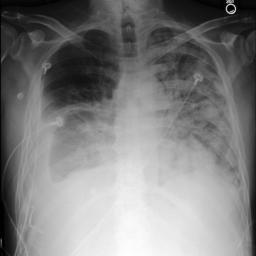
\includegraphics[width=0.24\textwidth]{./images/vqvae_recon/orig/000000_5391944b-b54dc685-7e6f258e-4af54573-0cfe07a5.jpg} &
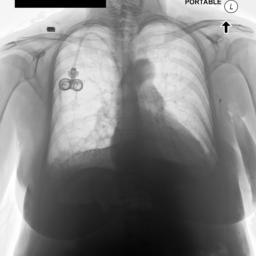
\includegraphics[width=0.24\textwidth]{./images/vqvae_recon/orig/000002_fa22acbe-44e11685-f7500129-c8243d38-b60af2f4.jpg} &
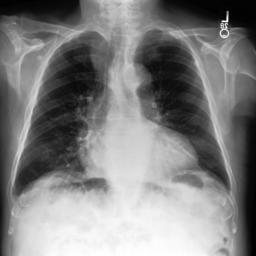
\includegraphics[width=0.24\textwidth]{./images/vqvae_recon/orig/000004_a5c5a35a-bbf9d41e-11d16b10-6369a012-9b46414a.jpg} &
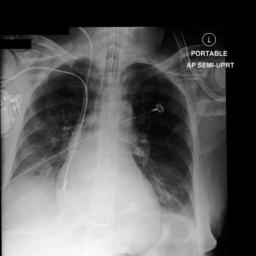
\includegraphics[width=0.24\textwidth]{./images/vqvae_recon/orig/000006_67ba7fde-43d98cc3-cd6efcf2-af65980f-e3daeb17.jpg} \\

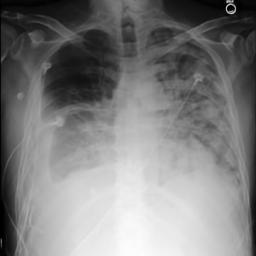
\includegraphics[width=0.24\textwidth]{./images/vqvae_recon/recon/000000_5391944b-b54dc685-7e6f258e-4af54573-0cfe07a5.jpg} &
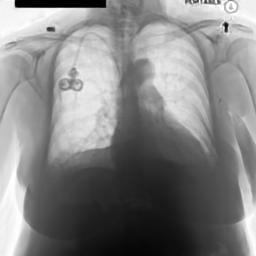
\includegraphics[width=0.24\textwidth]{./images/vqvae_recon/recon/000002_fa22acbe-44e11685-f7500129-c8243d38-b60af2f4.jpg} &
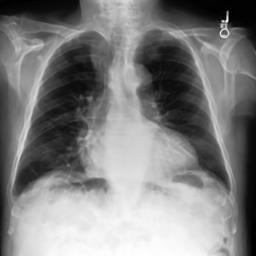
\includegraphics[width=0.24\textwidth]{./images/vqvae_recon/recon/000004_a5c5a35a-bbf9d41e-11d16b10-6369a012-9b46414a.jpg} &
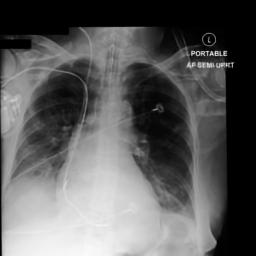
\includegraphics[width=0.24\textwidth]{./images/vqvae_recon/recon/000006_67ba7fde-43d98cc3-cd6efcf2-af65980f-e3daeb17.jpg} \\
\end{tabular}

\caption{Top row: original CXRs. Bottom row: corresponding VAE reconstructions.}
\label{fig:vae_orig_vs_recon_4}
\end{figure}